\documentclass[conference]{IEEEtran}
\IEEEoverridecommandlockouts
\usepackage{cite}
\usepackage{amsmath,amssymb,amsfonts}
\usepackage{graphicx}
\usepackage{textcomp}
\usepackage{xcolor}
\usepackage{float}
\usepackage{subcaption}
\usepackage{booktabs}

\def\BibTeX{{\rm B\kern-.05em{\sc i\kern-.025em b}\kern-.08em
    T\kern-.1667em\lower.7ex\hbox{E}\kern-.125emX}}

\begin{document}

\title{A Multimodal Digital Twin Framework for Alzheimer's Disease Progression and Prediction}

\author{
\IEEEauthorblockN{Mihit Singasane, Ved Thakker, Ria Talsania}
\IEEEauthorblockA{Department of Computer Engineering \\
Sardar Patel Institute of Technology \\
Guide: Prof. Swapnali Kurhade}
}

\maketitle

\begin{abstract}
Alzheimer's disease (AD) is a progressive, biologically diverse neurodegenerative condition whose diagnosis increasingly requires the integration of structural neuroimaging, molecular biomarkers, cognitive testing, and clinical observation. Traditional single-modality diagnostic pipelines cannot adequately capture this complexity, leading to poor risk stratification and delayed detection. This paper presents a Multimodal Digital Twin Framework for Alzheimer's Disease that fuses three complementary machine-learning pipelines: (1) a CatBoost clinical classifier trained on 2{,}149 structured lifestyle, cognitive, functional, and physiological records, achieving 96\% accuracy; (2) a ResNet34 convolutional neural network trained on 44{,}000 skull-stripped MRI scans, reaching 99.7\% accuracy on four-way dementia-stage classification; and (3) a biomarker--genotype ensemble (XGBoost + Random Forest + Neural Network, Optuna-blended) combining CSF ABETA, TAU, MMSE, APOE genotype, and MRI-derived volumetrics, achieving 63.3\% accuracy on an independent ADNI holdout set. A vision-language OCR module (Groq LLaMA-4 Maverick) converts unstructured medical reports into standardized JSON, enabling automated real-world data ingestion across all pipelines. The outputs are fused into a patient-specific Digital Twin that provides risk profiles, stage classification, and multimodal, interpretable insights, laying the groundwork for precision treatment planning and longitudinal disease-progression modeling.
\end{abstract}

\begin{IEEEkeywords}
Digital Twin, Alzheimer's Disease, Multimodal Fusion, CatBoost, ResNet34, ADNI, Biomarkers, APOE Genotype, OCR, Vision-Language Model
\end{IEEEkeywords}

\section{Introduction}
Alzheimer's Disease (AD) is a progressive neurodegenerative disorder affecting memory, cognition, and daily functioning, and remains one of the foremost healthcare challenges of the 21st century. Conventional diagnostic workflows rely on late-stage clinical symptoms or structural MRI changes that emerge only after substantial neurodegeneration has already occurred, delaying intervention and reducing therapeutic effectiveness.

\subsection{The Need for Multimodal AI in Alzheimer's Diagnosis}
Single-modality diagnostic techniques carry significant drawbacks: genetic and biomarker tests do not reflect functional or cognitive status; MRI reveals only structural damage after major neurodegeneration; and clinical evaluation alone cannot capture underlying biological pathology. AD is fundamentally multifactorial, spanning amyloid deposition, tau accumulation, neuroinflammation, metabolic dysfunction, and cognitive decline, each with distinct timescales and detection modalities. Digital Twin technology addresses this by maintaining a continuously updated virtual replica of a patient across clinical, imaging, genetic, and biomarker domains, enabling earlier detection, trajectory simulation, and individualized treatment planning.

\subsection{Problem Statement}
Most existing Alzheimer's diagnostic techniques rely on late-stage symptoms, and no comprehensive framework currently integrates MRI imaging, genetic/biomarker data, and clinical parameters into a single, dynamic, decision-support-capable Digital Twin.

\subsection{Objectives}
\begin{itemize}
    \item Develop a multimodal Digital Twin architecture for AD using heterogeneous datasets.
    \item Implement clinical ML models for Alzheimer's classification.
    \item Build an MRI-based deep learning model to classify dementia stages (NonDemented, VeryMild, Mild, Moderate).
    \item Construct a biomarker- and genotype-based risk prediction model.
    \item Integrate multimodal outputs into a unified Digital Twin representation.
    \item Develop an OCR-based medical report extraction system for automated data ingestion.
\end{itemize}


\section{Literature Survey}
Venugopalan et al.\ \cite{venugopalan2021} pioneered multimodal AD research, combining MRI, clinical scores, and genetic markers via autoencoders and 3D-CNNs, though their approach relied on single time-point data with limited interpretability. Chen et al.\ \cite{chen2022} used an attention-based CNN-Transformer for state-of-the-art MRI classification but did not integrate molecular biomarkers. Dolci et al.\ \cite{dolci2024} proposed a GAN-driven multimodal fusion framework to handle missing modalities, improving interpretability but remaining limited to cross-sectional diagnosis. Venkatraghavan et al.\ \cite{phd_debm} introduced the Disease Evolution Based Model (DEBM), mapping population-level biomarker timelines rather than personalized trajectories.

Bertolini et al.\ \cite{bertolini2021} developed a Conditional RBM-based Digital Twin for cognitive decline modeling are an early step toward patient-specific modeling but required complete multimodal data, which is rare clinically. Amato et al.\ \cite{amato2025} used EEG-based Digital Twins to estimate biomarker levels non-invasively without MRI or genetic integration. Lee et al.\ \cite{lee2023} and Sprint et al.\ \cite{sprint2024} demonstrated that large language models could extract cognitive biomarkers from speech, though restricted to progression modeling. Wu et al.\ \cite{wu2022} introduced federated learning for privacy-preserving AD model training across hospitals, though performance remained bound by ADNI's modality-completeness requirements.

\subsection{Research Gap}
Existing literature rarely unifies clinical, neuroimaging, and molecular-genetic dimensions into a single patient representation, and most work is restricted to snapshot classification rather than longitudinal modeling. Practical issues such as incomplete data, unstructured report formats, and the need for automated ingestion  are seldom addressed. This work directly targets these gaps by combining clinical CatBoost predictions, MRI deep learning, a biomarker--genotype ensemble, and OCR-driven data extraction into one Digital Twin structure, laying groundwork for future progression forecasting and treatment simulation.

\section{Methodology}

\subsection{System Architecture}
The proposed system uses three parallel prediction pipelines — Clinical, MRI, and Biomarker — whose outputs are fused into a unified patient Digital Twin, with an OCR layer digitizing unstructured medical reports for automated ingestion (Fig.~\ref{fig:architecture}).

\begin{figure}[H]
    \centering
    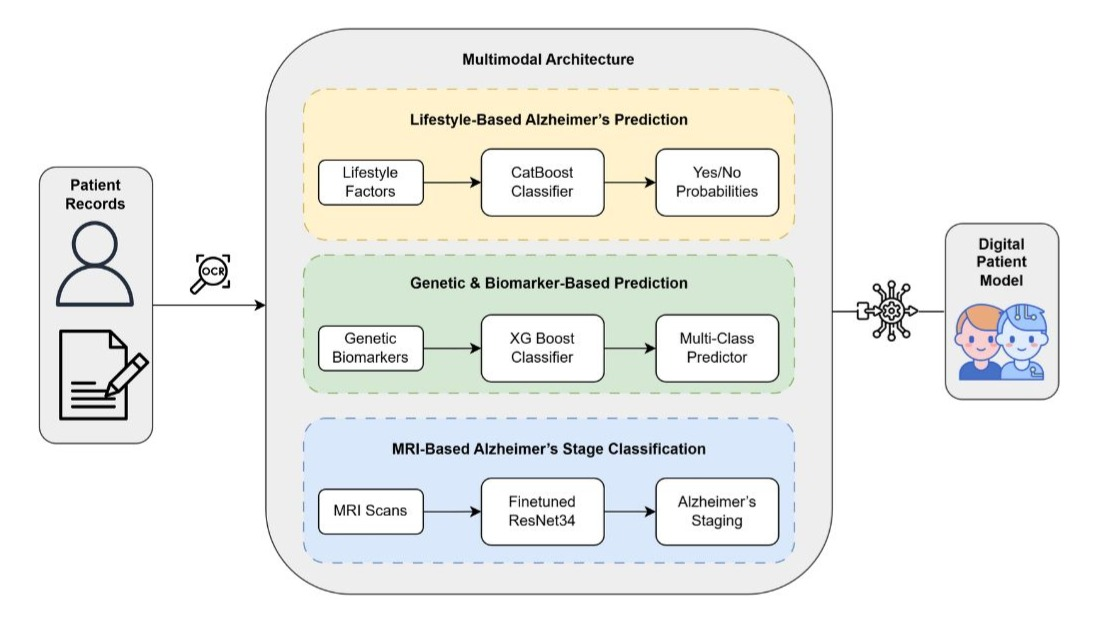
\includegraphics[width=0.9\linewidth]{System Architecture.JPG}
    \caption{Overall architecture showing the three parallel prediction pipelines and their fusion into a unified patient Digital Twin.}
    \label{fig:architecture}
\end{figure}

\begin{figure}[H]
    \centering
    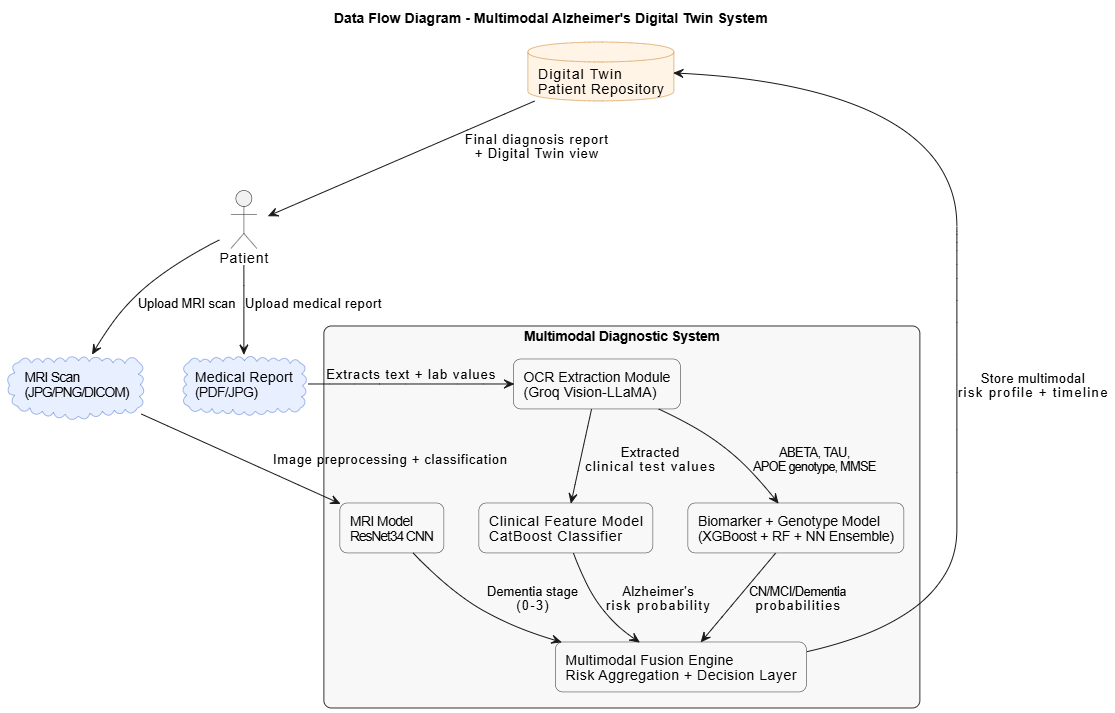
\includegraphics[width=0.9\linewidth]{Data Flow for Alzheimers.drawio.png}
    \caption{Data flow from medical reports, MRI scans, and lab results through OCR extraction, preprocessing, and model inference to Digital Twin output.}
    \label{fig:dataflow}
\end{figure}

\subsection{Clinical Model: CatBoost Classification}
The clinical pipeline used 2{,}149 patient records (Kaggle Alzheimer's Dataset) with 33 numerical features spanning demographics, lifestyle, medical history, vitals, cholesterol metrics, cognitive/functional tests, and behavioral indicators, with a binary Diagnosis target (65\% negative, 35\% positive). After dropping non-predictive identifiers, correlation analysis identified Functional Assessment ($-0.36$), ADL ($-0.33$), and MMSE ($-0.24$) as the strongest negative predictors, and Memory Complaints ($+0.30$) and Behavioral Problems ($+0.22$) as the strongest positive predictors. Fifteen continuous features were scaled using MinMaxScaler followed by StandardScaler, and the data was split 80--20 with a fixed random seed (42).

Seven algorithms were benchmarked using GridSearchCV (5-fold, F1-scoring): Decision Tree, Random Forest, KNN, Logistic Regression, SVM, XGBoost, and CatBoost. The final CatBoostClassifier (iterations$=100$, learning\_rate$=0.01$, depth$=6$, eval\_metric$=$F1, random\_seed$=42$) outperformed all alternatives, forming the first diagnostic layer of the Digital Twin.

\subsection{MRI Model: Dementia Stage Classification (ResNet34)}
The MRI pipeline classifies severity into NonDemented, VeryMildDemented, MildDemented, and ModerateDemented using $\sim$44{,}000 skull-stripped MRI scans (12{,}800 / 11{,}200 / 10{,}000 / 10{,}000 images respectively), sourced from an upsampled, augmented Kaggle MRI dataset. Preprocessing included resizing, pixel normalization to $[0,1]$, and augmentation (random rotation, zoom, horizontal flip, lighting adjustment) via fastai's \texttt{DataBlock} and \texttt{ImageDataLoaders}.

A transfer-learning ResNet34 backbone (\texttt{vision\_learner(dls, resnet34, metrics=[accuracy, error\_rate])}) was fine-tuned for five epochs, with a softmax head for four-class prediction. This forms the neuroimaging layer of the patient's Digital Twin.

\subsection{Biomarker + Genotype Ensemble Model}
CSF biomarkers, MRI-derived volumetrics, cognitive scores, and APOE genotype were sourced from the ADNI (Alzheimer's Disease Neuroimaging Initiative) consolidated table (\texttt{ADNIMERGE\_13Aug2025.csv}), extracting ABETA, TAU, MMSE, and APVOLUME, merged via patient RID with a one-hot-encoded APOE genotype table (\texttt{GENOTYPE\_3\_3}, \texttt{GENOTYPE\_3\_4}, \texttt{GENOTYPE\_2\_3}, \texttt{GENOTYPE\_4\_4}, \texttt{GENOTYPE\_2\_4}). The merged dataset contained $\sim$3{,}000 patient rows with a three-class diagnostic target: CN (Cognitively Normal), MCI (Mild Cognitive Impairment), and Dementia.

Engineered features included \texttt{ABETA\_TAU\_RATIO} (amyloid--tau balance) and \texttt{MMSE\_TAU\_INTERACT} (cognitive-tau coupling), yielding an 11-column feature matrix. Preprocessing applied median imputation, StandardScaler normalization, PCA retaining 98\% variance, and SMOTE oversampling (training set only) to address class imbalance (Dementia $<$ MCI $<$ CN).

Three base learners were trained on the PCA-transformed feature space:
\begin{itemize}
    \item \textbf{XGBoost}: learning\_rate$=0.05$, max\_depth$=7$, n\_estimators$=300$, subsample$=0.9$, colsample\_bytree$=0.9$
    \item \textbf{Random Forest}: n\_estimators$=400$, max\_depth$=14$, min\_samples\_split$=4$
    \item \textbf{Neural Network (MLP)}: hidden layers $(256,128,64)$, ReLU, Adam, max\_iter$=500$
\end{itemize}

Optuna optimized the blending weights $w_{xgb}, w_{rf}, w_{nn}$ for
\[
p_{\text{blend}} = w_{xgb}\, p_{xgb} + w_{rf}\, p_{rf} + w_{nn}\, p_{nn},
\]
yielding $w_{xgb}=0.6109$, $w_{rf}=0.3498$, $w_{nn}=0.0392$, confirming XGBoost as the dominant contributor.

\subsection{OCR Model for Automated Report Extraction}
An OCR module built on Groq's Vision-LLaMA (\texttt{llama-4-maverick-17b-128e-instruct}) parses uploaded medical reports (PDFs, images, scans) into structured JSON. Report images are base64-encoded and passed to the vision model under a strict medical-report-parser prompt, extracting patient information, report metadata, test results (name, value, unit, reference range), and clinical notes/diagnoses/medications when visible; missing fields are returned as \texttt{"N/A"}. Extracted values such as ABETA, TAU, MMSE, and APOE genotype feed the biomarker model; vitals and cognitive scores feed the CatBoost clinical model; MRI images bypass OCR and feed the MRI classifier directly making OCR the unified data-ingestion layer of the Digital Twin.

\subsection{Multimodal Fusion and Digital Twin Structure}
Each modality's predictions and confidence scores are standardized and reported alongside one another for interpretability. The Digital Twin itself is a JSON object containing demographics, clinical evaluation (CatBoost output), MRI analysis (dementia stage), biomarker measurements with APOE genotype, OCR-extracted fields, fused diagnosis and risk score, and a temporal history array  updated at every clinical visit to support future longitudinal trajectory analysis.

\section{Results and Discussion}

\subsection{Clinical Model Results}
Correlation analysis (Fig.~\ref{fig:pearson}) confirmed Functional Assessment, ADL, and MMSE as the strongest negative predictors of AD diagnosis, and Behavioral Problems and Memory Complaints as the strongest positive predictors.

\begin{figure}[H]
    \centering
    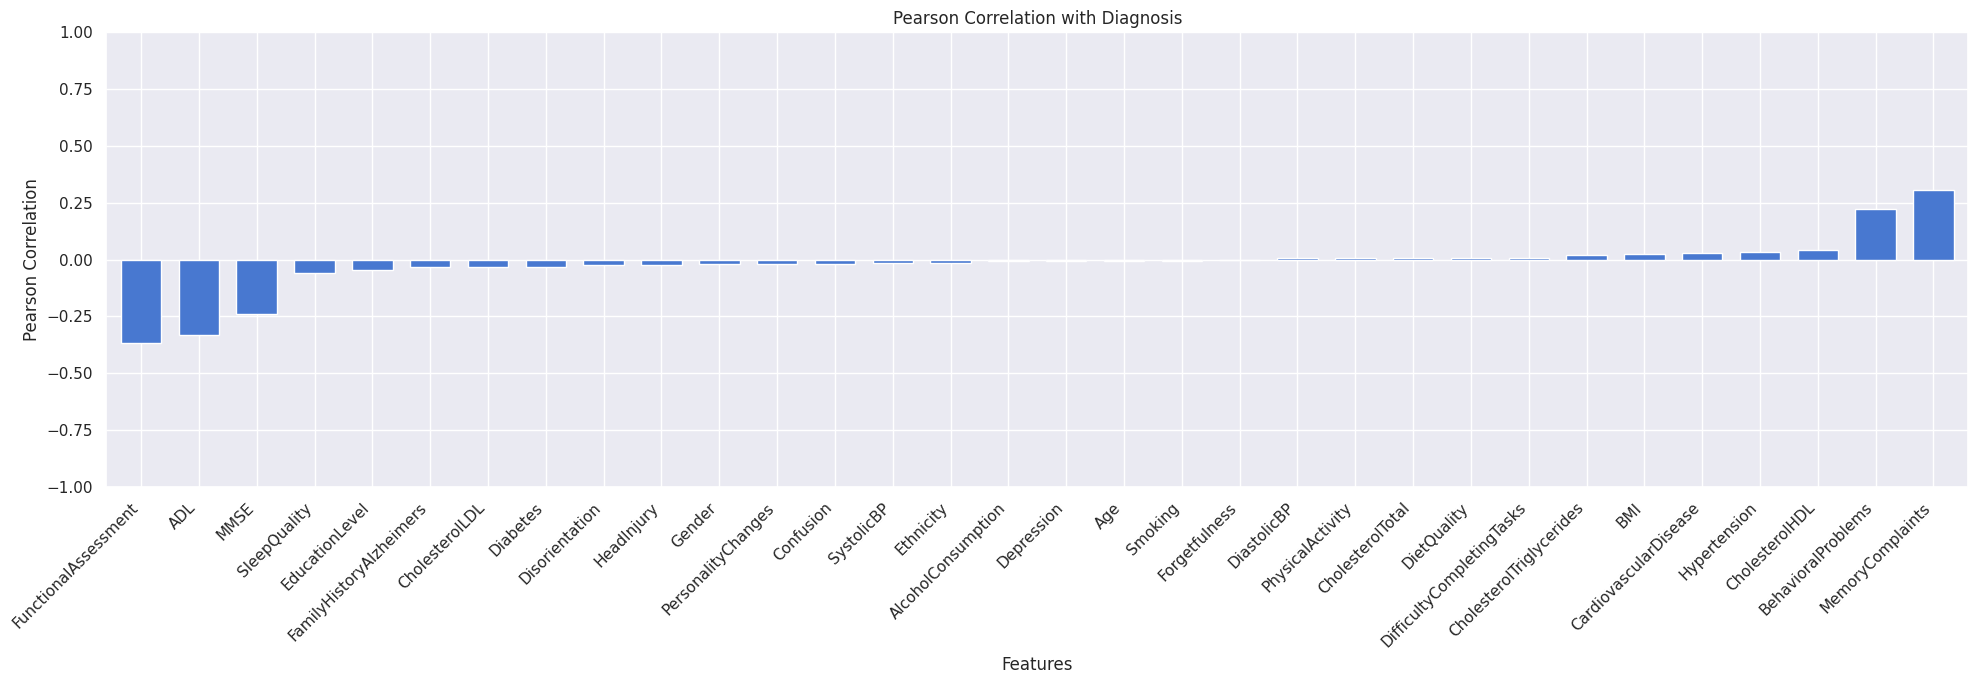
\includegraphics[width=0.95\linewidth]{pearson.png}
    \caption{Pearson correlation of clinical features with diagnosis label.}
    \label{fig:pearson}
\end{figure}

\begin{table}[H]
\centering
\caption{Clinical Model Performance Comparison}
\begin{tabular}{@{}lcccc@{}}
\toprule
\textbf{Model} & \textbf{Acc.} & \textbf{Prec.} & \textbf{Rec.} & \textbf{F1} \\
\midrule
Decision Tree & 0.93 & 0.92 & 0.87 & 0.90 \\
Random Forest & 0.92 & 0.96 & 0.80 & 0.88 \\
KNN & 0.72 & 0.68 & 0.61 & 0.54 \\
Logistic Regression & 0.83 & 0.79 & 0.71 & 0.75 \\
SVM & 0.83 & 0.81 & 0.73 & 0.77 \\
XGBoost & 0.95 & 0.94 & 0.91 & 0.93 \\
\textbf{CatBoost} & \textbf{0.96} & \textbf{0.96} & \textbf{0.92} & \textbf{0.94} \\
\bottomrule
\end{tabular}
\label{tab:clinical}
\end{table}

CatBoost achieved the best generalization overall (Table~\ref{tab:clinical}) and was selected as the clinical-stage classifier for the Digital Twin.

\subsection{MRI Classification Results}
The ResNet34 model improved steadily across five epochs, reaching 99.72\% validation accuracy (Table~\ref{tab:mri}), with near-perfect separation between dementia stages and only minor confusion between adjacent severity classes (Fig.~\ref{fig:mri_cm}).

\begin{table}[H]
\centering
\caption{MRI Model Training Performance}
\begin{tabular}{@{}cccc@{}}
\toprule
\textbf{Epoch} & \textbf{Train Loss} & \textbf{Valid Loss} & \textbf{Accuracy} \\
\midrule
0 & 0.2629 & 0.3385 & 0.8710 \\
1 & 0.1287 & 0.0930 & 0.9656 \\
2 & 0.0445 & 0.0316 & 0.9885 \\
3 & 0.0094 & 0.0129 & 0.9950 \\
4 & 0.0028 & 0.0084 & 0.9972 \\
\bottomrule
\end{tabular}
\label{tab:mri}
\end{table}

\begin{figure}[H]
    \centering
    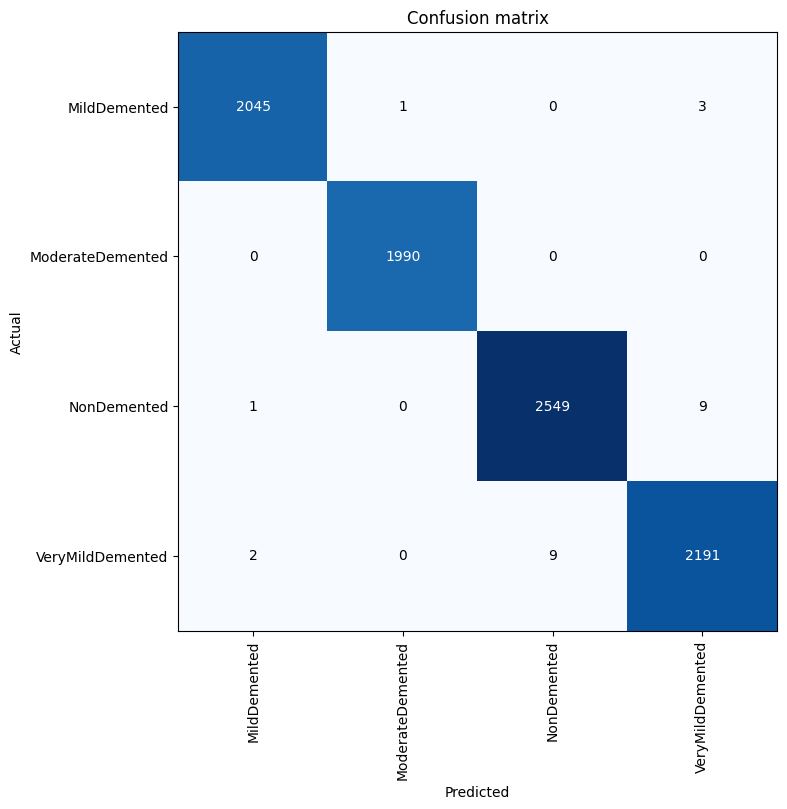
\includegraphics[width=0.85\linewidth]{Confusion matrix for image.png}
    \caption{Confusion matrix for the ResNet34 MRI classifier on the holdout set (8{,}800 images), achieving 99.7\% accuracy.}
    \label{fig:mri_cm}
\end{figure}

\subsection{Biomarker + Genotype Ensemble Results}
On the independent ADNI holdout set (1{,}716 samples), the Optuna-blended ensemble achieved overall accuracy 0.633 and weighted F1 0.63 (Table~\ref{tab:biomarker}). Dementia showed the strongest recall (0.77) due to distinct tau and volumetric signatures, while MCI was the hardest class to separate from CN owing to overlapping biomarker ranges (Fig.~\ref{fig:bio_cm}).

\begin{table}[H]
\centering
\caption{Biomarker Model Performance Metrics}
\begin{tabular}{@{}lcccc@{}}
\toprule
\textbf{Class} & \textbf{Prec.} & \textbf{Rec.} & \textbf{F1} & \textbf{Support} \\
\midrule
CN & 0.61 & 0.71 & 0.66 & 601 \\
Dementia & 0.69 & 0.77 & 0.73 & 367 \\
MCI & 0.62 & 0.50 & 0.55 & 748 \\
\midrule
\textbf{Overall} & \textbf{0.64} & \textbf{0.63} & \textbf{0.63} & \textbf{1,716} \\
\bottomrule
\end{tabular}
\label{tab:biomarker}
\end{table}

\begin{figure}[H]
    \centering
    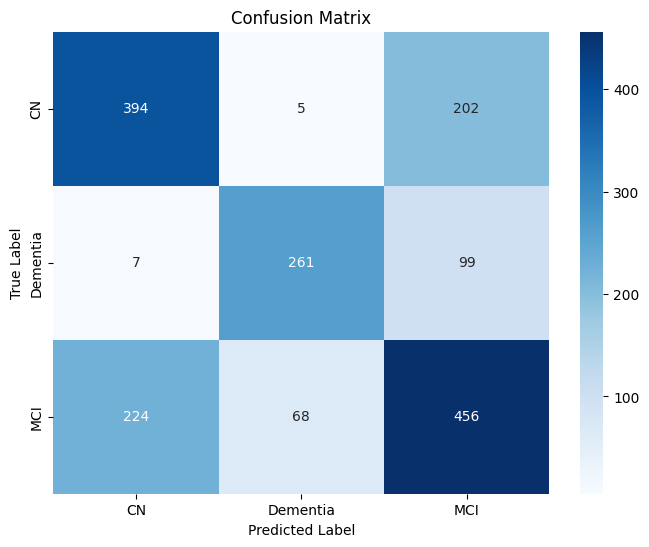
\includegraphics[width=0.75\linewidth]{Confusion matrix for gene.png}
    \caption{Confusion matrix for the biomarker--genotype ensemble, showing MCI overlap with CN and Dementia.}
    \label{fig:bio_cm}
\end{figure}

A holdout accuracy of 0.633 is consistent with published biomarker-only ADNI models: CSF biomarker ranges overlap substantially across CN, MCI, and dementia; the $\sim$3{,}000-sample dataset constrains neural-network performance; and APOE genotype is more informative for population-level risk than individual classification.

\subsection{Summary}
The Clinical CatBoost model achieved the highest tabular accuracy (0.96); the MRI ResNet34 model achieved near-perfect accuracy (0.997); and the Biomarker--Genotype ensemble achieved 0.633 accuracy despite limited sample size and biological overlap. Together with the OCR ingestion layer, each pipeline contributes a distinct diagnostic dimension like early functional decline, structural degeneration, and biological/genetic risk forming a multimodal, patient-specific foundation for the Digital Twin.

\section{Conclusion and Future Scope}
This work established a multimodal Digital Twin framework for Alzheimer's disease that integrates clinical, neuroimaging, and biomarker--genotype pipelines with automated OCR-based data ingestion. The CatBoost clinical classifier, ResNet34 MRI model, and Optuna-blended biomarker ensemble together demonstrate that complementary modalities can be unified into a single, interpretable patient-specific representation, validating the feasibility of Digital Twin technology for AD diagnostics.

Future work will extend this system toward temporal modeling: longitudinal data integration across visits, LSTM/GRU-based progression prediction, multimodal temporal transformers combining MRI, biomarkers, and OCR-extracted notes, treatment and intervention simulation, incorporation of larger ADNI cohorts, and eventual deployment as a full Clinical Decision Support System (CDSS) offering real-time risk assessment and personalized recommendations.

\begin{thebibliography}{99}

\bibitem{venugopalan2021}
S. Venugopalan, S. Tong, and R. K. Gupta, ``Multimodal deep learning for Alzheimer's disease diagnosis using MRI, genetic, and clinical data,'' \textit{IEEE J. Biomed. Health Inform.}, 2021.

\bibitem{chen2022}
L. Chen, Y. Xie, and M. Liu, ``Attention-guided hybrid CNN-transformer for MRI-based Alzheimer's classification,'' \textit{Neurocomputing}, 2022.

\bibitem{dolci2024}
A. Dolci et al., ``Interpretable multimodal fusion using GANs for Alzheimer's classification,'' \textit{Frontiers in Neuroscience}, 2024.

\bibitem{phd_debm}
A. Venkatraghavan, ``Disease Evolution Based Modeling (DEBM) for Alzheimer's disease progression,'' \textit{IEEE Trans. Med. Imaging}, 2018.

\bibitem{bertolini2021}
N. Bertolini et al., ``Digital twins for simulating Alzheimer's cognitive decline using CRBMs,'' \textit{Nature Sci. Rep.}, 2021.

\bibitem{amato2025}
C. Amato et al., ``EEG-driven digital twins for non-invasive prediction of Alzheimer's disease biomarkers,'' \textit{IEEE Trans. Neural Syst. Rehabil. Eng.}, 2025.

\bibitem{lee2023}
H. Lee et al., ``Conversational biomarkers using LLMs for detecting cognitive impairment,'' \textit{Nature Aging}, 2023.

\bibitem{sprint2024}
G. Sprint et al., ``Language perplexity as a digital biomarker for Alzheimer's and MCI,'' \textit{Alzheimer's \& Dementia}, 2024.

\bibitem{wu2022}
Y. Wu et al., ``A federated learning framework for privacy-preserving Alzheimer's diagnosis,'' \textit{IEEE Access}, 2022.

\bibitem{catboost2018}
L. Prokhorenkova et al., ``CatBoost: unbiased boosting with categorical features,'' \textit{NeurIPS}, 2018.

\bibitem{xgboost2016}
T. Chen and C. Guestrin, ``XGBoost: A scalable tree boosting system,'' \textit{Proc. ACM SIGKDD}, 2016.

\bibitem{rf2001}
L. Breiman, ``Random Forests,'' \textit{Machine Learning}, 2001.

\bibitem{fastai2019}
J. Howard and S. Gugger, ``FastAI: A layered API for deep learning,'' \textit{Information}, 2019.

\bibitem{adni_database}
ADNI Consortium, ``Alzheimer's Disease Neuroimaging Initiative (ADNI) dataset,'' adni.loni.usc.edu, Accessed 2025.

\bibitem{kaggle_mri}
Uraninjo, ``Augmented Alzheimer MRI Dataset V2,'' Kaggle, 2024.

\bibitem{kaggle_clinical}
Kaggle, ``Alzheimer's Clinical Dataset,'' Kaggle, 2023.

\bibitem{groq_llama}
Groq Inc., ``LLaMA 4 Maverick Vision Model Documentation,'' 2025.

\bibitem{ocr_medical2024}
A. Saha et al., ``OCR systems for structured medical report extraction,'' \textit{IEEE Access}, 2024.

\end{thebibliography}

\end{document}